\chapter{Guest Speaker David Swensen: The Yale Model and Long-Horizon Investing}

This guest lecture, delivered by David Swensen in Robert J. Shiller's Financial Markets course and curated here by LazyingArt LLC, begins with a criticism rather than a theorem. Barron's had treated Yale's endowment strategy as too aggressive, too illiquid, and insufficiently diversified. Swensen's reply is not a slogan. He reconstructs the portfolio world he inherited in 1985, separates the sources of return into asset allocation, market timing, and security selection, and then argues that a well-diversified, equity-oriented portfolio is the right expression of long-horizon institutional investing.

\section{The Yale model under criticism}

Robert J. Shiller introduces Swensen by stressing two facts at once. First, Swensen had an unusual Wall Street pedigree: he had been involved in the early swap market. Second, he had managed Yale's endowment from less than one billion dollars in 1985 to roughly \$16.7 billion by June 2010. The lecture therefore opens with authority already established. What changes the tone is that this authority arrives in the aftermath of the financial crisis, when Yale's success is being openly challenged.

Swensen leans into that challenge. He notes that publicity had once been uniformly favorable, with commentators praising either the ``Yale model'' or the ``Swensen approach.'' After Lehman and the crisis, the headlines turned. Barron's argued that endowments should hold more conventional stocks and bonds and less in alternatives because the alternatives did not provide enough diversification and did not provide enough liquidity. That criticism supplies the problem for the whole lecture: what is the Yale model, and are those two objections actually correct?

The lecture's first important move is therefore methodological. Swensen does not begin by defending alternatives directly. He first asks what kind of portfolio a long-horizon institution ought to hold, and only then returns to the crisis-era criticism.

\section{1985 endowments and two failed tests}

Swensen's answer begins by going backward. When he arrived at Yale in 1985, he did the obvious thing: he looked around to see how other sophisticated institutions were investing. What he found was an endowment world with a remarkably conventional structure:
\begin{equation}
\left(w_{\text{US stocks}},\,w_{\text{US bonds+cash}},\,w_{\text{alternatives}}\right)
\approx (0.50,\,0.40,\,0.10).
\end{equation}
The lecture treats this allocation as failing two basic tests. The first is diversification. The second is equity orientation.

On diversification, Swensen invokes the finance theory associated with Tobin and Markowitz. He does not derive mean-variance theory in detail, but the lecture's point is the standard one: diversification is a free lunch in the sense that one can improve the return-risk tradeoff without changing the underlying investment horizon. In standard notation, if two portfolios have the same expected return, the diversified one can have lower variance,
\begin{equation}
E[R_p]=E[R_q], \qquad \sigma^2(R_p)<\sigma^2(R_q),
\end{equation}
and conversely, for a given level of variance, the diversified one can have a higher expected return,
\begin{equation}
\sigma^2(R_p)=\sigma^2(R_q), \qquad E[R_p]>E[R_q].
\end{equation}

Swensen's claim is that the inherited endowment portfolio was not diversified in any serious sense. A portfolio with half its assets in a single asset class is concentrated. Worse, with roughly ninety percent in U.S. marketable securities, it is exposed to a narrow set of common drivers. His concrete example is interest rates. Lower interest rates are good for bonds by direct discounting; lower discount rates also raise the present value of future earnings streams and can therefore support stock prices as well. The lecture does not write a board formula here, but the standard present-value expressions make the point precise:
\begin{align}
P_{\text{bond}} &= \sum_{t=1}^{T}\frac{C_t}{(1+r)^t}+\frac{F}{(1+r)^T},\\
P_{\text{equity}} &= \sum_{t=1}^{\infty}\frac{CF_t}{(1+r)^t}.
\end{align}
If the same discount-rate movement can improve both sides of the portfolio, then the portfolio is less diversified than it first appears.

The second failure is equity orientation. Swensen argues that an endowment, unlike almost any other investor, has a genuinely long horizon. Its mandate is not simply to avoid short-run volatility. It is to preserve purchasing power in perpetuity. That mandate should make the institution a natural bearer of equity risk. Yet the standard mid-1980s portfolio held about forty percent in bonds and cash, which Swensen treats as low expected return assets. In his terms, the old endowment structure failed both the common-sense diversification test and the common-sense equity test.

\subsection{Question \& Answer}

\paragraph{Question.} If diversification was already basic finance theory, why were endowments still so badly structured?

\paragraph{Answer.} The lecture's answer is institutional rather than abstract. Swensen arrives, looks at peer institutions, and discovers that practice has congealed into a convention. Portfolios are being copied and inherited, not rebuilt from first principles. The result is a structure that sounds prudent because it is conventional, but once we inspect it carefully it is neither well diversified nor appropriately designed for a perpetual investor.

\section{Three tools of return}

Having diagnosed the old world, Swensen introduces the lecture's main analytical framework. There are, he says, three things an investor can do to affect returns.

First, one can choose what assets to own and in what proportions. That is asset allocation.

Second, one can deviate from long-run targets because of a short-run view. That is market timing.

Third, one can try to beat the market inside an asset class by overweighting some securities and underweighting others. That is security selection.

The lecture becomes much clearer once these three levers are separated. For note-writing purposes, the clean decomposition is
\begin{equation}
R_p = R_{\text{policy}} + \alpha_{\text{timing}} + \alpha_{\text{selection}} - L,
\end{equation}
where \(R_{\text{policy}}\) is the return generated by the long-run policy portfolio, the two \(\alpha\) terms are returns from active deviations, and \(L\) collects the leakages of active investing: fees, commissions, market impact, taxes, and similar costs.

\begin{figure}[h]
\centering
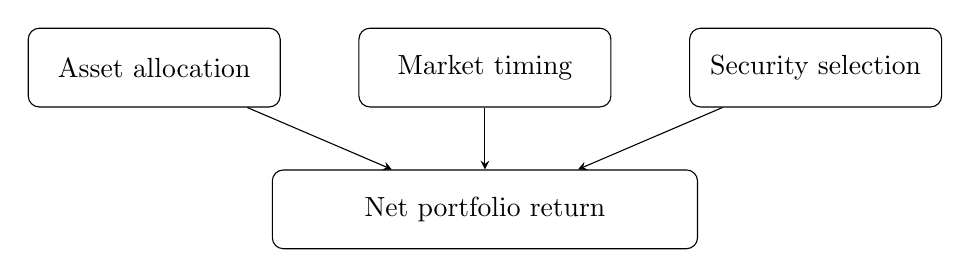
\begin{tikzpicture}[>=stealth]
\node[draw, rounded corners, minimum width=3.2cm, minimum height=1cm] (a) at (0,1.6) {Asset allocation};
\node[draw, rounded corners, minimum width=3.2cm, minimum height=1cm] (b) at (4.2,1.6) {Market timing};
\node[draw, rounded corners, minimum width=3.2cm, minimum height=1cm] (c) at (8.4,1.6) {Security selection};
\node[draw, rounded corners, minimum width=5.4cm, minimum height=1cm] (d) at (4.2,-0.2) {Net portfolio return};
\draw[->] (a) -- (d);
\draw[->] (b) -- (d);
\draw[->] (c) -- (d);
\end{tikzpicture}
\end{figure}

The next claim is subtle. Swensen says asset allocation is ``far and away'' the most important tool, but then immediately refuses to treat that as a metaphysical law of finance. If Yale's entire endowment were put into Google stock, security selection would dominate. If the whole endowment were used to day-trade bond futures, market timing would dominate. These examples sound silly, and that is their point. Real investors do not usually behave that way. They tend to keep a stable policy portfolio, and within each asset class they tend to diversify. Under those behavioral conditions, asset allocation becomes the primary determinant of return variation.

This is why Swensen can cite the Ibbotson result that more than ninety percent of the variability of institutional returns is attributable to asset allocation, and then go further. If timing and selection are negative-sum after costs on average, then the policy allocation can explain more than one hundred percent of net returns:
\begin{equation}
\overline{\alpha_{\text{timing}}}+\overline{\alpha_{\text{selection}}}-\overline{L}<0.
\end{equation}
The active terms do not merely fail to help. On average they subtract from what a passive implementation of policy would have delivered.

\subsection{Question \& Answer}

\paragraph{Question.} Why can asset allocation dominate returns even though market timing and security selection also exist?

\paragraph{Answer.} Because the dominance claim is conditional on ordinary investment behavior. Once we assume that investors keep a stable policy mix and hold diversified portfolios inside each asset class, the remaining movements in total return are driven mainly by the asset-class exposures themselves. The extreme cases in which timing or selection dominate are logically possible but behaviorally abnormal.

\section{Long horizons, equity risk, and the small-stock temptation}

Swensen now turns from structure to long-run evidence. Using Roger Ibbotson's historical data, he compares what would have happened to one dollar invested from the end of 1925 to 2009. The lecture emphasizes not annual averages but long-run wealth accumulation:
\begin{align}
M_{\text{bills}} &= 21, &
M_{\text{inflation}} &= 12,\\
M_{\text{bonds}} &= 86, &
M_{\text{large stocks}} &= 2592,\\
M_{\text{small stocks}} &= 12226. &&
\end{align}
The intended inference is clear. If we move out along the risk spectrum from Treasury bills to bonds to equities, long-run wealth rises dramatically. A perpetual investor should therefore accept substantial equity exposure.

But the lecture does not stop with that conclusion. It immediately raises a more dangerous one. If small stocks produce the highest long-run multiple by a huge margin, why not simply put the whole portfolio into small stocks and be done with it? Swensen presents this as a live temptation. It would even make life simpler for an investment committee: just buy the one thing with the best historical record and forget the rest.

\subsection{Question \& Answer}

\paragraph{Question.} If small stocks dominate the long-run data, why not put the whole endowment into small stocks?

\paragraph{Answer.} Because long-run dominance does not tell us whether a strategy is survivable. Swensen's answer is the Great Depression. If the entire portfolio sits in small stocks at the peak, then the path of losses is catastrophic:
\begin{align}
W_{1929} &= W_0(1-0.54)=0.46W_0,\\
W_{1930} &= 0.46W_0(1-0.38)=0.2852W_0,\\
W_{1931} &= 0.2852W_0(1-0.50)=0.1426W_0,\\
W_{1932} &= 0.1426W_0(1-0.32)\approx 0.097W_0.
\end{align}
So the dollar at the peak becomes roughly ten cents at the trough. At that point the issue is no longer theoretical expected return. It is whether any investor, individual or institutional, can actually remain invested. Swensen's answer is no. Heavy equity exposure is sensible for a long-horizon investor, but concentration in one risky segment is not.

This is where the lecture's tone shifts from pure compounding arithmetic to institutional psychology. The historical memory of market collapse was so intense, he notes, that many fiduciaries came to regard heavy equity exposure as irresponsible. Diversification therefore re-enters the story not as a decorative add-on but as the condition that makes an equity-oriented strategy livable through frightening periods.

\section{Market timing and security selection as negative-sum behavior}

The next lever is market timing. Swensen introduces it through a Keynes quotation: those who try to buy and sell large shifts in markets tend to sell too late, buy too late, and do both too often, thereby increasing risk while paying heavy expenses. The lecture then supplies empirical evidence for that claim.

Morningstar compared time-weighted returns and dollar-weighted returns for U.S. domestic equity mutual funds. The logic is simple. Time-weighted returns tell us how the fund performed. Dollar-weighted returns tell us how investors experienced it once the timing of cash inflows and outflows is taken into account. In every one of the seventeen categories in the study,
\begin{equation}
R^{DW}<R^{TW}.
\end{equation}
The interpretation is that investors systematically add money after strong performance and pull money out after weak performance. They buy high and sell low.

Swensen then sharpens the point with the internet-fund example. The reported time-weighted return across the top internet funds over the six-year window around the bubble was only modestly positive, about \(1.5\%\) per year. Yet investors reportedly put in about \$13.7 billion and lost about \$9.5 billion. The point is not the exact arithmetic of the episode; the transcript itself is rough at that level. The point is the pattern. Investors did not hold those funds evenly through the whole period. They piled in near the top and sold in disappointment after the collapse.

Institutions do not escape this logic. Swensen's example is October 1987. Stocks fell violently; government bonds rallied in a flight to safety. The portfolio implication was straightforward: equities had become cheaper and bonds more expensive. Yet institutions sold stocks and bought bonds. Endowments then took years to rebuild equity allocations, remaining underweight in the heart of a powerful bull market. The lecture's general claim is therefore broad: both individual and institutional investors are tempted to chase performance, and market timing is the mechanism through which that temptation damages returns.

The same negative-sum logic appears in security selection. Inside an asset class, if we simply buy the market index, then there is no active selection return:
\begin{equation}
\alpha_{\text{selection}}=0.
\end{equation}
If instead we overweight Ford and underweight GM relative to the market, then some other investor must be on the other side. Before costs, aggregate active return sums to zero:
\begin{equation}
\sum_i \alpha^{\text{selection}}_i = 0.
\end{equation}
After costs, it becomes negative:
\begin{equation}
\sum_i \left(\alpha^{\text{selection}}_i-L_i\right) < 0.
\end{equation}
Swensen applies similar reasoning, more cautiously, to timing in the aggregate. The community of investors cannot all overweight the same asset class relative to target without offsetting positions elsewhere. Once the cost of playing is added, timing too becomes negative-sum on average.

\subsection{Question \& Answer}

\paragraph{Question.} If active management is zero-sum before costs, why does the average active investor still lose?

\paragraph{Answer.} Because the game is not played for free. Swensen lists commissions, market impact, manager fees, consultant fees, loads, and taxes. He then adds survivorship bias. A cited study gives only about a \(14\%\) chance of beating the market after fees and taxes. But that figure already excludes front-end loads and is biased toward surviving funds. Once dead funds are counted, the success rate moves toward zero. The lecture's conclusion is not that nobody ever wins. It is that the average investor confronts a structurally losing game.

\section{Where active management matters}

Up to this point, Swensen has shown why active management is dangerous in the aggregate. He now asks a sharper question: where, if anywhere, is active effort worth spending?

His proposed practical proxy is dispersion. If a market is highly efficient, then managers should cluster near the benchmark. Large departures from market return should be rare and unstable. If a market is less efficient, the spread between strong and weak managers should be wider. The lecture therefore uses the cross-manager return spread within an asset class as a guide to where skill might matter most:
\begin{align}
\Delta_{\text{bonds}} &\approx 0.5\% \text{ per year},\\
\Delta_{\text{large cap}} &\approx 2.0\% \text{ per year},\\
\Delta_{\text{foreign}} &\approx 4.0\% \text{ per year},\\
\Delta_{\text{absolute return}} &\approx 7.1\% \text{ per year},\\
\Delta_{\text{real estate}} &\approx 3.0\% \text{ per year},\\
\Delta_{\text{LBO}} &\approx 13.7\% \text{ per year},\\
\Delta_{\text{VC}} &\approx 43.2\% \text{ per year}.
\end{align}

The interpretation is one of the lecture's most distinctive institutional claims. Bonds are ``just math'': coupons, principal, and default probabilities. That makes them relatively easy to analyze and therefore relatively efficient. In such markets the manager's safest response is to hug the benchmark. Venture capital is different. There may not even be a benchmark that can be mechanically matched. One cannot index a collection of idiosyncratic private partnerships in the same way one indexes large-cap public equities. There the spread between excellent and poor managers is large, and manager selection becomes much more consequential.

This is not a general defense of every alternative asset. It is a narrower claim. If active management is costly everywhere, then it should be concentrated where the opportunity set is widest.

\section{Barron's revisited, and the institutional application}

With the framework complete, Swensen returns to the original criticism. On diversification, he concedes a narrow point: in a panic, diversification can fail. When markets collapse into a binary distinction between risk and safety, many risky assets are sold together and U.S. Treasuries are bought together. In that short window, the only asset that really diversifies is the safe asset everyone wants.

But this concession is not a surrender. To hold a large Treasury allocation all the time is to pay an opportunity cost year after year. A portfolio with \(25\%\), \(30\%\), or \(35\%\) in Treasuries may feel clever during a panic and expensive in ordinary times. Swensen therefore shifts the horizon back to where he thinks it belongs. Over long stretches, underinvestment in risky productive assets is costly. Over equally long stretches, country concentration is also costly, which is why he brings in Japan:
\begin{equation}
\text{Nikkei}_{1989}\approx 38{,}000,\qquad \text{Nikkei}_{2009}\approx 10{,}500,
\end{equation}
so that the cumulative loss is roughly
\begin{equation}
1-\frac{10{,}500}{38{,}000}\approx 73\%.
\end{equation}
A long horizon by itself is not enough. One still needs diversification.

On the second Barron's criticism, the alleged overemphasis on alternatives, Swensen responds with Yale's actual record over the decade ending June 30, 2010. Domestic equities had returned about \(-0.7\%\) per year and bonds about \(5.9\%\). Alternatives, by contrast, produced substantially stronger figures in the cases he lists: private equity around \(6.2\%\), real estate \(6.9\%\), absolute return \(11.1\%\), timber \(12.1\%\), and oil and gas \(24.7\%\). The lecture's argument here is blunt. If the criticism is that alternatives were a mistake, the decade-level return comparison does not support it.

The final audience questions then refine the lecture's practical message rather than changing it. Swensen distinguishes Yale from individual investors on three margins. First, Yale is tax exempt; individuals are not, and taxes are a major drag on realized returns. Second, Yale can bring serious human capital to bear on manager selection; most individuals and many institutions cannot. Third, Yale sits one layer above the underlying securities and must solve a principal-agent problem: how to identify and contract with external managers so that they act in the university's interest.

For investors without Yale's resources, Swensen's advice is almost the opposite of the Yale model in its institutional form. Such investors should choose a sensible asset allocation and implement it passively through index funds. That is why his two books point in different directions: institutions with exceptional scale and expertise can attempt to exploit wide dispersion where skill matters, while ordinary investors should avoid paying active fees for mediocre active results.

\subsection{Question \& Answer}

\paragraph{Question.} If diversification fails during panics, why should a long-term investor still insist on it?

\paragraph{Answer.} Because panic is not the whole investment problem. The relevant comparison is not ``How did the portfolio behave in the worst few months?'' but ``What portfolio best preserves purchasing power over long horizons without forcing catastrophic concentration?'' Diversification may disappoint in moments of universal flight to safety, but concentration can destroy wealth over decades. Japan is Swensen's counterexample to the view that panic failure invalidates diversification.

The Q\&A also yields a useful operational rule. Swensen suggests that a well-diversified portfolio might have something like a \(5\%\) to \(10\%\) minimum allocation and a \(25\%\) to \(30\%\) maximum allocation to any single asset class. That rule matters because it supports a disciplined rebalancing policy. If actual weights drift away from policy targets, then
\begin{equation}
w_i \to w_i^{*}.
\end{equation}
The rule is simple but powerful. Suppose domestic equities have underperformed and a \(20\%\) target has drifted down to \(16\%\). Rebalancing means buying the missing four percentage points and funding that purchase by trimming assets that have outperformed. If equities have instead rallied and risen above target, rebalancing means selling them back down toward target. This is not heroic forecasting. It is a mechanical way of buying relative weakness and trimming relative strength while keeping risk exposure aligned with policy.

One further warning closes the lecture. Swensen is skeptical of simple Sharpe-ratio comparisons across institutional portfolios:
\begin{equation}
\text{Sharpe}=\frac{E[R_p-R_f]}{\sigma(R_p)}.
\end{equation}
His objection is not to the algebra. It is to the measurement. Marketable securities are marked continuously and display high short-run volatility. Illiquid assets such as timber and real estate are appraised infrequently, and appraisal smoothing mechanically dampens measured standard deviation. Two portfolios can therefore produce numerically comparable Sharpe ratios while embodying risks that are not comparable at all. In his language, this becomes an apples-and-oranges problem.

\section{Summary}

Swensen's lecture is built as a defense, but it becomes more than a defense. The Yale model is not simply a taste for alternatives. It is a way of organizing institutional investing around three propositions. First, long-horizon investors should be equity oriented. Second, they should be genuinely diversified rather than conventionally diversified. Third, once we separate policy allocation from timing and security selection, we see that most active behavior is costly and often self-defeating.

The lecture's final balance is careful. Diversification can fail in a panic, but it remains indispensable over long horizons. Active management is negative-sum on average, but it may still be worthwhile in markets with unusually wide dispersion if the institution has exceptional resources. And for investors without those resources, the right lesson is not imitation of Yale's institutional machinery but disciplined passive implementation of a sensible policy portfolio.